% !TEX TS-program = XeLaTeX
% use the following command: 
% all document files must be coded in UTF-8
\documentclass[spanish]{textolivre}
% See more information on the repository: https://github.com/leolca/textolivre

% Metadata
\begin{filecontents*}[overwrite]{article.xmpdata}
    \Title{Tendencias en el estado del arte de las narrativas audiovisuales móviles en el siglo XXI: revisión sistemática de la literatura}
    \Author{Valeriano Durán Manso \sep María-Victoria Carrillo-Durán \sep Javier Trabadela-Robles}
    \Language{es}
    \Keywords{tendencias \sep narrativas \sep audiovisual \sep dispositivos móviles \sep revisión sistemática}
    \Journaltitle{Texto Livre}
    \Journalnumber{1983-3652}
    \Volume{14}
    \Issue{3}
    \Firstpage{1}
    \Lastpage{16}
    \Doi{10.35699/1983-3652.2021.29457}

    \setRGBcolorprofile{sRGB_IEC61966-2-1_black_scaled.icc}
            {sRGB_IEC61966-2-1_black_scaled}
            {sRGB IEC61966 v2.1 with black scaling}
            {http://www.color.org}
\end{filecontents*}

\journalname{Texto Livre}
\thevolume{14}
\thenumber{3}
\theyear{2021}
\receiveddate{\DTMdisplaydate{2021}{2}{14}{-1}} % YYYY MM DD
\accepteddate{\DTMdisplaydate{2021}{4}{14}{-1}}
\publisheddate{\DTMdisplaydate{2021}{7}{23}{-1}}
% Corresponding author
\corrauthor{Javier Trabadela-Robles}
% DOI
\articledoi{10.35699/1983-3652.2021.29457}
%\articleid{NNNN} % if the article ID is not the last 5 numbers of its DOI, provide it using \articleid{} commmand
% Abbreviated author list for the running footer
\runningauthor{Durán Manso et al.}
\sectioneditorname{Daniervelin Pereira}
\layouteditorname{Anna Izabella M. Pereira}


\title{Tendencias en el estado del arte de las narrativas audiovisuales móviles en el siglo XXI: revisión sistemática de la literatura}
\othertitle{Tendências no estado da arte das narrativas audiovisuais móveis no século XXI: revisão sistemática da literatura}
\othertitle{Trends in the state of the art of mobile audiovisual narratives in the 21st century: systematic review of the literature}
% if there is a third language title, add here:
%\othertitle{Artikelvorlage zur Einreichung beim Texto Livre Journal}

\author[1]{Valeriano Durán Manso \orcid{0000-0001-9188-6166} \thanks{Email: \url{valerioduran@us.es}}}
\author[2]{María-Victoria Carrillo-Durán \orcid{0000-0002-1256-8870} \thanks{Email: \url{vicduran@unex.es}}}
\author[2]{Javier Trabadela-Robles \orcid{0000-0001-5338-9257} \thanks{Email: \url{jtrarob@unex.es}}}

\affil[1]{Universidad de Sevilla, Facultad de Comunicación, Departamento de Comunicación Audiovisual y Publicidad, Sevilla, Andalucía, España.}
\affil[2]{Universidad de Extremadura, Facultad de Ciencias de la Documentación y la Comunicación, Departamento de Información y Comunicación, Badajoz, Extremadura, España.}

\addbibresource{article.bib}
% use biber instead of bibtex
% $ biber tl-article-template

% set language of the article
\setdefaultlanguage{spanish}
\setotherlanguage{portuguese}
\setotherlanguage{english}

% for spanish, use:
%\setdefaultlanguage{spanish}
%\gappto\captionsspanish{\renewcommand{\tablename}{Tabla}} % use 'Tabla' instead of 'Cuadro'
%\AfterEndPreamble{\crefname{table}{tabla}{tablas}\Crefname{table}{Tabla}{Tablas}}

% for languages that use special fonts, you must provide the typeface that will be used
% \setotherlanguage{arabic}
% \newfontfamily\arabicfont[Script=Arabic]{Amiri}
% \newfontfamily\arabicfontsf[Script=Arabic]{Amiri}
% \newfontfamily\arabicfonttt[Script=Arabic]{Amiri}
%
% in the article, to add arabic text use: \textlang{arabic}{ ... }

% to use emoticons in your manuscript
% https://stackoverflow.com/questions/190145/how-to-insert-emoticons-in-latex/57076064
% using font Symbola, which has full support
% the font may be downloaded at:
% https://dn-works.com/ufas/
% add to preamble:
% \newfontfamily\Symbola{Symbola}
% in the text use:
% {\Symbola }

% reference itens in a descriptive list using their labels instead of numbers
% insert the code below in the preambule:
\makeatletter
\let\orgdescriptionlabel\descriptionlabel
\renewcommand*{\descriptionlabel}[1]{%
  \let\orglabel\label
  \let\label\@gobble
  \phantomsection
  \edef\@currentlabel{#1\unskip}%
  \let\label\orglabel
  \orgdescriptionlabel{#1}%
}
\makeatother
%
% in your document, use as illustraded here:
%\begin{description}
%  \item[first\label{itm1}] this is only an example;
%  % ...  add more items
%\end{description}
 

% custom epigraph - BEGIN 
%%% https://tex.stackexchange.com/questions/193178/specific-epigraph-style
\usepackage{epigraph}
\renewcommand\textflush{flushright}
\makeatletter
\newlength\epitextskip
\pretocmd{\@epitext}{\em}{}{}
\apptocmd{\@epitext}{\em}{}{}
\patchcmd{\epigraph}{\@epitext{#1}\\}{\@epitext{#1}\\[\epitextskip]}{}{}
\makeatother
\setlength\epigraphrule{0pt}
\setlength\epitextskip{0.5ex}
\setlength\epigraphwidth{.7\textwidth}
% custom epigraph - END


% if you use multirows in a table, include the multirow package
\usepackage{multirow}

% add line numbers for submission
%\usepackage{lineno}
%\linenumbers

\begin{document}
\maketitle

\begin{polyabstract}
\begin{abstract}
La investigación sobre narrativas audiovisuales móviles como productos de ficción ha tenido una presencia irregular en la bibliografía científica del siglo XXI. La rápida expansión de los dispositivos móviles ha favorecido sus posibilidades, apareciendo inicialmente series específicas para este soporte, las denominadas moviseries. En este trabajo se ha realizado un análisis bibliográfico sistemático, desde 2000 a 2018, de las principales bases de datos, WOS, Scopus y Google Scholar, mediante una selección de palabras clave que definen el objeto de estudio: moviseries, nuevas narrativas, \emph{storytelling}, series de televisión. Del corpus inicial de 750 referencias, se filtraron 36 trabajos correspondientes a las Ciencias Sociales, y, en concreto, a la categoría de Comunicación. En los resultados se muestran, primero, los diversos enfoques de los trabajos. Por una parte, existen trabajos de corte descriptivo que hablan de las estructuras narrativas, su origen y evolución (enfoque predominante), por otra parte, existen trabajos realizados desde el ámbito educativo, que inciden en la percepción y los hábitos de consumo del usuario, por último, están los trabajos realizados desde la dimensión tecnológica. En segundo lugar, se extraen resultados sobre las metodologías empleadas. A este respecto, sobresalen los trabajos de carácter cualitativo y los estudios de caso. En tercer lugar, se extraen conclusiones sobre el estado de la cuestión en distintos países. Desde estas consideraciones, la internacionalización es una pauta dominante, si bien los artículos realizados por autores de universidades de un mismo país son más numerosos que las colaboraciones internacionales. 

\keywords{Tendencias \sep Narrativas \sep Audiovisual \sep Dispositivos móviles \sep Revisión sistemática}
\end{abstract}

\begin{portuguese}
\begin{abstract}
A investigação sobre narrativas audiovisuais móveis como produtos ficcionais tem tido uma presença irregular na literatura científica do século XXI. A rápida expansão dos dispositivos móveis tem favorecido suas possibilidades como oportunidade de negócio para a indústria do entretenimento, surgindo inicialmente séries específicas para este meio, as chamadas moviseries. Neste artigo, foi realizada uma análise bibliográfica sistemática, de 2000 a 2018, das principais bases de dados, WOS, Scopus e Google Scholar, através de uma selecção de palavras-chave que definem o objecto de estudo: moviseries, novas narrativas, contos, séries televisivas. Do corpus inicial de 750 referências, 36 trabalhos correspondentes às Ciências Sociais, e especificamente, à categoria de Comunicação, foram filtrados. Os resultados mostram, em primeiro lugar, as diferentes abordagens dos trabalhos. Por um lado, existem trabalhos descritivos que falam sobre estruturas narrativas, sua origem e evolução (abordagem predominante), por outro lado, existem trabalhos realizados a partir do campo educacional, que se concentram na percepção e hábitos de consumo do usuário e, finalmente, existem trabalhos realizados a partir da dimensão tecnológica. Em segundo lugar, são extraídos resultados sobre as metodologias utilizadas. A este respeito, destacam-se os estudos qualitativos e os estudos de caso. Em terceiro lugar, são tiradas conclusões sobre o estado da questão em diferentes países. A partir destas considerações, a internacionalização é um padrão dominante, embora os artigos de autores de universidades do mesmo país sejam mais numerosos do que as colaborações internacionais.

\keywords{Tendências \sep Narrativas \sep Audiovisual \sep Dispositivos móveis \sep Revisão sistemática}
\end{abstract}
\end{portuguese}

\begin{english}
\begin{abstract}
Research on mobile audiovisual narratives as fiction products has had an irregular presence in the scientific literature of the 21st century. The rapid expansion of mobile devices has fostered their possibilities, with the initial appearance of specific series for this medium, the so-called moviseries. In this work, a systematic analysis of the literature has been carried out (2000-2018) from the main databases, WOS, Scopus and Google Scholar, using a selection of keywords that define the object of study: moviseries, new narratives, storytelling and television series. From the initial corpus of 750 references, 36 research works corresponding to the Social Sciences, and specifically to the Communication category, were filtered out. The results show, first of all, the different approaches of the works. On one hand, there are descriptive works that talk about narrative structures, their origin and evolution (predominant approach), on the other hand, there are works carried out in the educational field, which focus on the user's perception and consumption habits, and finally, there are works carried out from the technological dimension. Secondly, results are drawn from the methodologies used. In this respect, qualitative studies and case studies stand out. Thirdly, conclusions are drawn on the state of the art in different countries. From these considerations, internationalisation is a dominant pattern, although articles by authors from universities in the same country are more numerous than international collaborations. 

\keywords{Trends \sep Narratives \sep Audiovisual \sep Mobile devices \sep Systematic review}
\end{abstract}
\end{english}

% if there is another abstract, insert it here using the same scheme
\end{polyabstract}


\section{Introducción}\label{sec-intro}
La investigación en narrativas audiovisuales en dispositivos móviles ha tenido una presencia irregular en la bibliografía académica de los últimos años. La rápida expansión entre los usuarios de diferentes soportes tecnológicos y sus posibilidades para transmitir productos audiovisuales, hizo que las industrias de la ficción y el ocio vieran en los móviles una importante –y emergente-, oportunidad de negocio \cite{barron2013, feijoo2010}. Sin embargo, lo que parecía un soporte que podría convertirse en una alternativa para nuevos productos seriados se fue convirtiendo en una plataforma para la emisión de los contenidos ya existentes en las televisiones generalistas \cite{saez2010}. Partiendo de esta situación, resulta pertinente observar la evolución de la investigación que se ha desarrollado desde el inicio del siglo XXI, sobre las narrativas audiovisuales móviles, como objeto de estudio que engloba los avances realizados sobre los contenidos de ficción específicos para dispositivos móviles. 

Así, se ha abordado la situación en países de habla hispana y anglosajones, tanto para tratar el desarrollo del propio objeto, como la forma de realizarse la investigación sobre el mismo (la metodología). Si bien es cierto que Europa es el continente donde más países han prestado atención a este tema, en Asia y en América, e incluso en África y en Oceanía –especialmente en Australia-, destacan interesantes focos académicos dedicados a su estudio \cite{shim2017, dawson2012, goggin2012}. El panorama internacional aporta pues una visión general del estado de la cuestión y permite examinar las diferentes realidades de esos países. 

Desde estas consideraciones, el objetivo general de este trabajo es conocer en qué momento se encuentra la investigación en narrativas audiovisuales móviles con contenidos de ficción seriada, específicos para dispositivos móviles y, también, la trayectoria académica de esta línea de investigación en el presente siglo, en revistas de impacto. Para ello, se plantean los siguientes objetivos específicos: 

\begin{itemize}
\item Realizar un análisis bibliográfico sistemático de las referencias sobre narrativas audiovisuales móviles presentes en las principales bases de datos: Web of Science (WOS), Scopus y Google Scholar, atendiendo a una selección de palabras clave que definen el objeto de estudio y que se explican más adelante: moviseries, nuevas narrativas, \emph{storytelling} y series de televisión.
\item Abordar las dimensiones temáticas del objeto de estudio y los planteamientos metodológicos desde los que ha sido tratado en los artículos que componen la revisión. 
\item Reflexionar sobre el carácter internacional de las investigaciones analizadas para conocer el origen y la procedencia de las universidades y centros de investigación que las han originado. 
\end{itemize}

\section{Justificación de la investigación y términos de búsqueda}
El siglo XXI trajo en su primera década la difusión de contenidos audiovisuales móviles \cite{gomez2007, urban2007, jumiskopyykko2008}. Esto supuso un interesante aspecto para las posibilidades de entretenimiento en estos terminales, llegando a configurarse conceptos específicos que definen un panorama nuevo para la narrativa audiovisual en dispositivos móviles. A continuación, se explican las palabras claves que abordan y describen el objeto de estudio y definen este nuevo panorama: 

Moviseries: este término aparece definido en la literatura de forma específica \cite{adelantadomateu2011, morante2011, saez2010} como aquellas series de ficción creadas y diseñadas específicamente para móviles. Este nuevo producto, que nació en 2003 en Estados Unidos \cite{dawson2012}, tuvo su máximo apogeo en España entre 2005 y 2010 con títulos como «Supervillanos» (La Sexta/ Globomedia, 2006) o «A pera picada» (TV3/ Lavinia, 2008), que, posteriormente, pasaron a emitirse en televisión. Como apunta \textcite{morante2011}, las moviseries presentan rasgos que pueden configurar un estilo audiovisual propio para la ficción en móviles, como la pantalla reducida –donde deben destacar los planos medios y cortos sobre los generales-, el color, los mensajes cortos o la duración de entre 1,5 y 3 minutos. A este respecto, la duración otorga identidad al relato, pues deben predominar historias breves que puedan ser consumidas rápidamente. 

Por ello, el autor señala que la consolidación del producto dependería del aprovechamiento de nuevas ventanas de difusión, la existencia de las tarifas planas de Internet y la alta velocidad, o de la creación de aplicaciones específicas para móviles, iPhone, Blackberry y Android. Además, como indican \textcite{mendiz-noguero2011}, existen espacios que resultan adecuados para el consumo de estos productos, todos vinculados con los periodos de espera, como los transportes o los bloques de anuncios de televisión, en los que los usuarios buscan elementos de distracción para pasar el tiempo. Estos rasgos dibujan un panorama en el que las moviseries parecen tener identidad propia \cite{prario2007}. El hecho de que se creara este concepto propició un tipo de producto determinado y definido que permitió a los teléfonos móviles convertirse en dispositivos difusores del mismo. 

Su antecedente directo es la webserie, que apareció en la literatura en 1997 \cite{saez2010}, en Estados Unidos, y alude a los contenidos seriados de ficción creados para emitirse por Internet \cite{monaghan2017, montoyabermudez2016, barron2013}. Las webseries presenciaron la aparición de las moviseries –que tuvieron un cierto auge en la primera década del siglo XXI-, pero experimentaron posteriormente un desarrollo más amplio, con productos como «Qué vida más triste» (La Sexta/ Mediapro, 2008) y «Becari@s» (Telecinco, 2008) \cite{saez2010}. Ambos formatos, surgidos por la presencia de Internet en la telefonía móvil, marcan el rumbo de los productos seriados de ficción en estos dispositivos, cambiando así los tradicionales hábitos de consumo de estos en las plataformas convencionales, condicionados también por las transformaciones tecnológicas de la industria de la telefonía móvil. 

Nuevas narrativas: los conceptos moviseries y webseries se engloban en las nuevas narrativas. Este término está ligado a las narrativas transmedia, un concepto que fue designado por \textcite{jenkins2003} para abordar la convergencia de medios y las posibilidades de los distintos canales en la expansión narrativa del relato \cite{scolari2013}. La narración móvil surgió en plena expansión de la convergencia mediática y puso de relieve las posibilidades de difusión y de expansión de los relatos mediante los teléfonos móviles \cite{rincon2011}, aportando un nuevo soporte a la creación y difusión de nuevas narrativas. 

\emph{Storytelling}: este término ha sido definido junto al de narrativa tratando de ver sus similitudes y diferencias. \textcite{lugmayr2017} proponen la definición de «\emph{serious storytelling}» cuando la narración busca un objetivo más allá del entretenimiento. Así, \emph{storytelling} hace referencia a la capacidad de contar, plantear y narrar historias, y «\emph{serious storytelling}» a la capacidad de intervenir en la obtención de un objetivo que puede ser estratégico y aplicable en la comunicación digital. Por tanto, en el escenario audiovisual actual esta palabra aparece ligada a las narrativas transmedia y se considera como una forma de nueva narrativa audiovisual, útil para fidelizar al público alrededor de un mundo narrativo \cite{scolari2017}. En cuanto a los dispositivos móviles, este concepto adquiere valor por constituir una manera de elaborar los argumentos, que se ajusta a la forma de contar pequeñas historias que tengan continuidad y que se pueden desarrollar en estos dispositivos, adaptando el relato a las características físicas de los aparatos tecnológicos \cite{morante2011}. 

Series de televisión: las narrativas audiovisuales móviles tienen su origen en los contenidos de ficción creados para las series de televisión, y los rasgos vinculados con sus construcciones narrativas derivan de ellas. Debido a esta simbiosis, algunas moviseries han sido trasladadas a la pequeña pantalla \cite{saez2010} y numerosas series han encontrado nuevas posibilidades de difusión en Internet \cite{adelantadomateu2011}. Este aspecto ha tenido más influencia en el ámbito de las webseries \cite{montoyabermudez2016, barron2013} por su desarrollo más constante frente a las moviseries. 

Por otra parte, la delimitación temporal de la investigación del objeto de estudio se concreta en los años transcurridos desde el comienzo del siglo XXI, puesto que se pretende conocer el estado del arte en el periodo en el que nacen y se desarrollan con éxito las moviseries. Este hecho presenta diferentes escenarios posibles en la investigación de las narrativas audiovisuales móviles y da lugar a una propuesta de partida para el trabajo. Por una parte, es posible que se justifique la existencia de una narrativa con características específicas para los soportes móviles –al margen de que el concepto moviserie no pareció desarrollarse de forma constante-, pero, por otra, es posible que las plataformas móviles se hayan convertido en instrumentos para difundir contenidos ya existentes en la televisión sin una conceptualización clara hasta la actualidad. 

Por tanto, se aborda el estudio de la literatura existente hasta la fecha en torno a las narrativas audiovisuales móviles, observando los diferentes ámbitos de estudio y la adaptación del tema a las diferentes realidades y países, lo que determinará el estado actual del objeto de estudio. 

\section{Material y métodos}
Para esta investigación se ha realizado un análisis sistemático de la literatura científica relativa al área de las Ciencias Sociales, y en concreto a la categoría de Comunicación, en los motores de búsquedas de WOS, Scopus y Google Scholar. Se han elegido estas tres bases de datos por su calidad científica contrastada (WOS y Scopus) y por su fácil acceso y popularidad (Google Scholar); este último es un instrumento claramente reconocido por la academia en su conjunto como un gran contenedor de información científica de gran aceptación dentro de la comunidad académico-científica \cite{maldonadomartinez2017} y donde además se encuentran la mayor parte de los trabajos ya indexados en WOS y JCR.

Aunque los smartphones se popularizan a comienzos de la segunda década del presente siglo, las búsquedas se realizan en el periodo que incluye desde el año 2000 al 2018. 

Se establecieron cuatro palabras clave introducidas en español y en inglés, vinculadas con el objeto de estudio y descritas más arriba: moviseries, nuevas narrativas, \emph{storytelling} y series de televisión. 

En la búsqueda se han contemplado los resultados arrojados teniendo en cuenta el criterio de coincidencia, lo que significa que los documentos más coincidentes con la palabra clave introducida aparecen primero. En este caso, se tuvieron en cuenta las 15 primeras páginas de cada una de las tres bases de datos, delimitando a 20 el número de artículos por página en WOS y Scopus y a 10 en el caso de Google Scholar. Así, se accedió a un total bruto de 750 artículos entre las tres bases de datos, siendo la muestra de análisis válida y final el resultado de la combinación de cada una de las palabras claves con cada una de las siguientes, de modo que, por ejemplo, la palabra moviserie fue combinada con nuevas narrativas/ \emph{storytelling}/ series de televisión e igual con todas las demás. De esta manera, se obtuvieron búsquedas parciales que puestas en común consiguieron filtrar los trabajos repetidos, siendo el resultado final un total de 36 documentos que se ajustaban con mayor precisión al objeto de estudio. 

De ellos, 32 son artículos y cuatro proceden de comunicaciones de congresos especializados en el área. En el primer caso, los artículos consultados pertenecen –en este orden-, a las siguientes revistas científicas del área de Comunicación: adComunica (España), Razón y Palabra (Mexico), Anagramas (Colombia), Comunicar (España), Anduli (España), L’Atalante (España), Observatorio (OBS) Journal (Portugal), Television \& New Media (Estados Unidos), Media International Australia (Australia), Computers in Human Behavior (Reino Unido), Journal of Computer Assisted Learning (Reino Unido), Journal of Advertising Research (Estados Unidos), Réseaux (Francia), Journal of Applied Research and Technology (México), Media, Culture and Society (Estados Unidos), Prisma Social (España), Palabra Clave (Colombia), Mediterranean Journal of Social Sciences (Italia), Popular Communication (Reino Unido), Journal Studies in Australasian Cinema (Reino Unido), El profesional de la información (España), Revista Comunicación (Colombia), Telematics and Informatics (Reino Unido), Journal of Media Business Studies (Reino Unido) y Convergence: The International Journal of Research into New Media Technologies (Reino Unido/ Estados Unidos). Comunicar, OBS, L’Atalante y Computers in Human Behavior cuentan con más de un artículo. 

En el segundo caso, las investigaciones se presentaron –en este orden–, en el II Congreso de la Asociación Española de Investigación de la Comunicación (AE-IC): «Comunicación y desarrollo en la era digital» (Málaga, 2010), IEEE Consumer Communications and Networking Conference (CCNC). The 8th Annual International Conference (Las Vegas, EEUU, 2011), MobileHCI '08 Proceedings of the 10th International Conference on Human Computer Interaction with Mobile Devices and Services (Nueva York, EEUU, 2008) y Proceedings of the Second International Workshop in Video Processing and Quality Metrics for Consumer Electronics (Scottsdale, EEUU, 2006). De esta manera, las revistas citadas y los eventos científicos celebrados evidencian la internacionalización en el tratamiento del objeto de estudio. 

En tercer lugar, se ha realizado un estudio de cada artículo aplicando una ficha de análisis con estos ítems: área / campo de estudio, principales temas, objetivos, metodología empleada y resultados / conclusiones. Estas categorías han permitido estructurar los trabajos que componen la muestra en función de las partes básicas que los conforman, lo que facilita el análisis de los contenidos. Los aspectos más representativos, y que constituyen los objetivos de este trabajo, son los siguientes: revisar el enfoque de estudio de cada artículo, el desarrollo metodológico utilizado, el origen geográfico de las autorías y la colaboración entre las universidades. Con este planteamiento, se puede establecer a nivel global qué ámbito –o ámbitos–, son los más recurrentes y habituales en las investigaciones sobre este tema; cuál –o cuáles-, son las principales tendencias metodológicas que se siguen; y, por último, qué investigadores y expertos son los que han profundizado en la cuestión y desde qué universidades –o centros de investigación-, valorando así, además, las contribuciones entre distintos países. Todo ello persigue conocer dónde están a nivel nacional e internacional los principales focos investigadores de la cuestión que se aborda: las narrativas audiovisuales móviles.  

\section{Análisis y resultados}
Según los objetivos planteados, se explican los resultados atendiendo a tres aspectos concretos: el ámbito temático o enfoque desde el que se ha realizado el trabajo, el planteamiento metodológico asumido y la distribución geográfica de la producción encontrada.

\subsection{Ámbito temático}
El corpus de análisis corresponde a las Ciencias Sociales, concretamente a la categoría de Comunicación, pero atiende a diversos enfoques que profundizan en las dimensiones del objeto de estudio, como el ámbito histórico-descriptivo, el ámbito tecnológico o el ámbito educativo y de hábitos de consumo (\Cref{fig1}). 

Aunque la búsqueda se realizó dentro del siglo XXI, fue entre 2007 y 2017 cuando se produjo una eclosión de estudios sobre estos nuevos formatos –especialmente desde un enfoque descriptivo e histórico–, que, si bien han indagado en las moviseries, después se han centrado en las webseries y, sobre todo, en las nuevas narrativas. Por ello, son numerosos los autores de diversa procedencia, como \textcite{adelantadomateu2011, barron2013, montoyabermudez2016, saez2010, dawson2012, orgad2009} –quien incluso habla del origen del concepto de «mobisodes», que son pequeños episodios de series para el móvil, es decir, los episodios de las moviseries-, o \textcite{jumiskopyykko2006}, que se han centrado en este aspecto, destacando los artículos que abordan las características y la estructura del objeto de estudio, así como la naturaleza de los productos seriados. Esta tendencia, que ahonda en el origen y el contexto del nacimiento del producto, es la más abundante. 

Asimismo, también han resultado interesantes aquellos artículos construidos en torno a otros enfoques, como el tecnológico, pues es importante conocer la dimensión técnica de los dispositivos móviles para poder profundizar en sus posibilidades narrativas, destacando los textos de \textcite{tamayofernandez2011, chuchu2014, jumiskopyykko2008} o \textcite{evens2011}.

En tercer lugar, están los artículos ligados al ámbito de la educación y hábitos de consumo de medios, como los enmarcados en la alfabetización digital, la educomunicación y el aprendizaje, destacando los de \textcite{phillippi-miranda2011, gomez2007, tornero2019, su2015, galindo2015}. Estos trabajos han realizado una aproximación a un aspecto necesario para conocer cómo las personas se enfrentan a los dispositivos móviles y saber cómo perciben sus productos narrativos. En esta línea, otros artículos centrados en los hábitos de consumo de los usuarios son los de \textcite{shim2017, figeac2009, do2009, goggin2012, urban2007}. 

El abordaje de los enfoques educativo/hábitos de consumo y tecnológico han tenido una presencia regular en estos años, pero el enfoque histórico-descriptivo presenta dos picos de atención, hacia 2011 y 2017. El primero corresponde al esfuerzo realizado para definir conceptos específicos como moviseries \cite{adelantadomateu2011, morante2011, saez2010} después de su popularización entre 2005 y 2010. El segundo parece ser un repunte ante el declive del esfuerzo en seguir teorizando sobre el objeto de estudio después de lo que parecía ser una etapa de auge a partir de 2011. 

\begin{figure}[htbp]
 \centering
 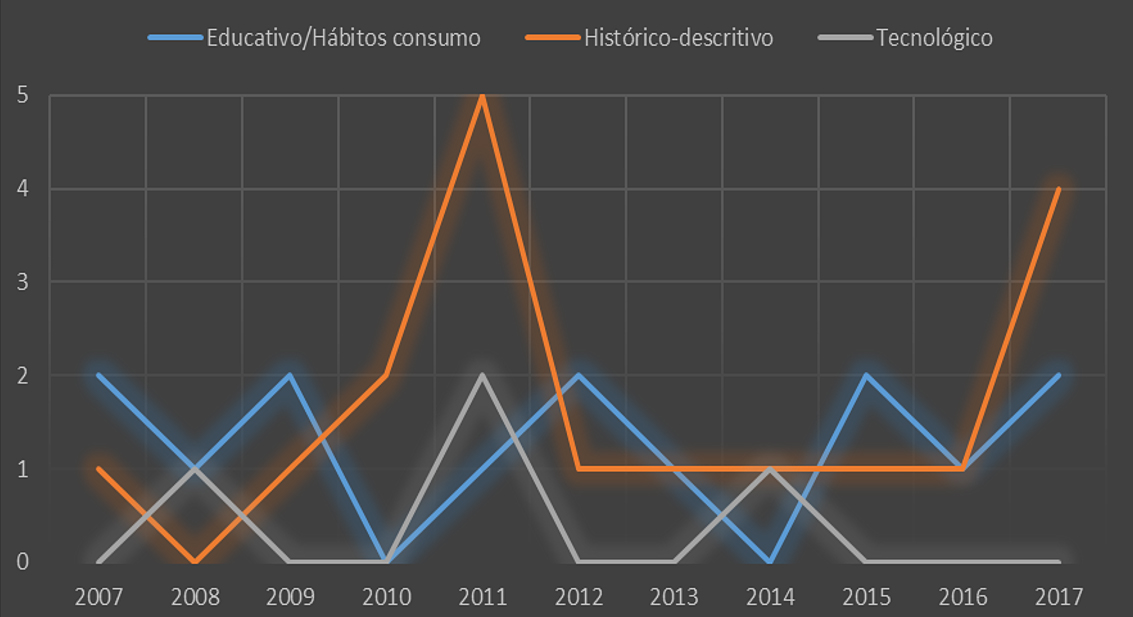
\includegraphics[width=0.9\textwidth]{fig-001[1].jpg}
 \caption{Distribución anual de los trabajos según el ámbito de estudio.}
 \label{fig1}
 \source{elaboración propia.}
\end{figure}

El análisis del ámbito temático es fundamental en la presente investigación, ya que las narrativas audiovisuales móviles han experimentado un rápido desarrollo a nivel mundial. Si bien es cierto que diversas investigaciones se centran en la aparición y la evolución histórica de las moviseries –sin duda, conocer el contexto se antoja fundamental para entender el producto–, por otra parte, el enfoque educativo/hábitos de consumo tampoco es mayoritario, y el enfoque tecnológico, tan importante para que el usuario pueda disfrutar de los contenidos, no cuenta con muchas investigaciones, siendo la tercera opción abordada en las investigaciones. La tecnología es fundamental puesto que una de las particularidades de estas narrativas es la adaptación al soporte móvil, lo que influye en el lenguaje audiovisual, en el tipo de planos que se emplean, la duración de los mismos o el desarrollo de los personajes, dado que el tamaño de la pantalla condiciona la recepción. Sin duda, el empleo y el uso de la tecnología posibilitan el desarrollo de los contenidos y determina la manera en que se accede a ellos y son visionados.

Por otra parte, en relación a las investigaciones en las que ha primado el ámbito educativo/hábitos de consumo, se puede decir que la forma en que se utilizan los dispositivos móviles y se consumen productos de ficción seriada ha alterado las habituales fórmulas de consumo. Ahora el receptor es también el usuario e interactúa con los contenidos. Los trabajos refieren ventajas e inconvenientes al acceso, directamente relacionadas con la tecnología y la forma de comercializarla, tales como el precio, la precariedad de los contenidos y dificultades de acceso desde los dispositivos móviles, entre otras. 

En resumen, se puede decir que el tratamiento del tema según diferentes ámbitos de estudio invita a reflexionar sobre los objetivos de las investigaciones, y se concluye que los autores han estudiado el nuevo entorno desde sus antecedentes y hasta su consolidación, han definido en menor medida las herramientas que lo han hecho posible y han explicado cómo los usuarios los han entendido y consumido desde un punto de vista pedagógico. 

\subsection{Planteamiento metodológico}
En cuanto a las metodologías empleadas para tratar el objeto de estudio, la muestra responde a dos líneas básicas (\Cref{fig2}). La primera se refiere a las metodologías de tipo cualitativo, predominando los estudios de caso \cite{martinezcarazo2006}. A este respecto, sobresalen países tan dispares como Australia \cite{varan2013, goggin2012}, Corea del Sur \cite{shim2017, do2009}, Taiwan \cite{su2015}, Malasia \cite{wong2016}, México \cite{tamayofernandez2011}, Sudáfrica \cite{chuchu2014}, Estados Unidos \cite{dawson2012}, Finlandia \cite{jumiskopyykko2008} e Italia \cite{prario2007}. También destacan estudios de caso sobre series de televisión de gran éxito en Internet y en el universo móvil, como «Morning Glory» y «Ciega a citas» (Mediaset, 2014) \cite{alonso2015}, «The Wire» (HBO, 2002/ 2008) \cite{mittell2017}, «The Good Wife» (CBS, 2009/ 2016) \cite{hargraves2017}, «Starting From…Now» (SBS2, 2014/ 2016) \cite{monaghan2017} o «El Ministerio del Tiempo» (TVE, 2015/ 2020) \cite{scolari2017}. 

En menor medida, algunos de los trabajos analizados se han realizado con metodologías cuantitativas. Este es el caso de los relativos a \textcite{shim2017, wong2016, su2015} –pertenecientes a investigaciones del continente asiático-, \textcite{lochrie2012, chuchu2014, jumiskopyykko2008}. En todos han predominado herramientas de recogida de información como cuestionarios o encuestas aplicando técnicas de análisis multivariable. No obstante, debido a la naturaleza del objeto de estudio, este tipo de metodologías no han sido tan numerosas como las cualitativas, donde en algunos casos se han utlizado formas de recogida de datos como entrevistas o focus group, o se han combinado con diseños mixtos (cualitativos y cuantitativos). Según los diferentes abordajes del objeto de estudio, los trabajos más numerosos pertenecen al enfoque histórico-descriptivo, que utilizan especialmente métodos cualitativos propios del mismo. Los trabajos relativos a la educación/hábitos y la tecnología presentan abordajes tanto cualitativos como cuantitativos o mixtos de forma equilibrada.

 \begin{figure}[htbp]
 \centering
 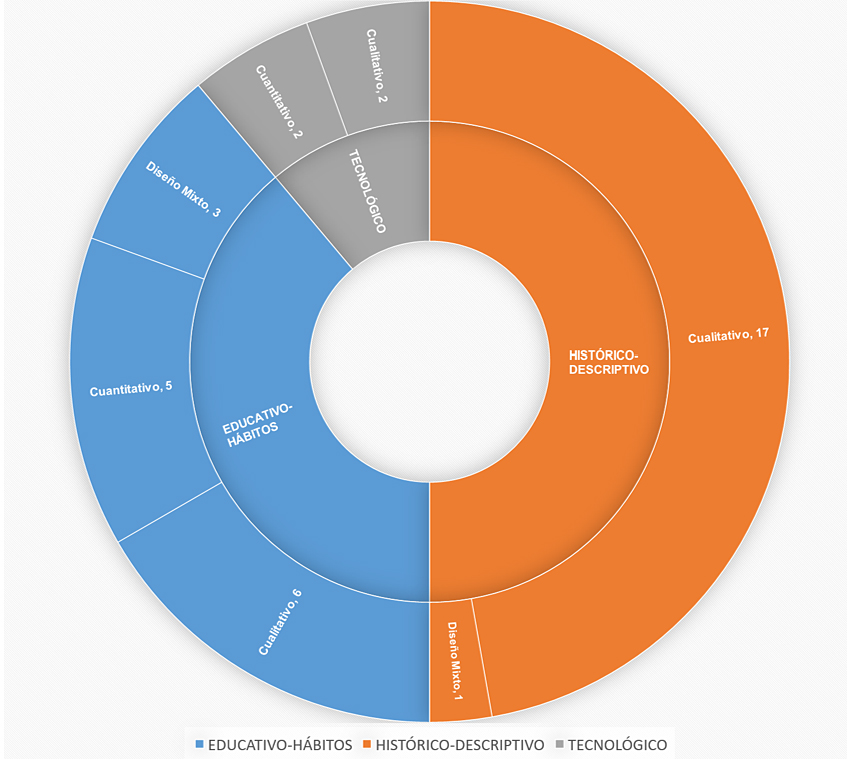
\includegraphics[width=\textwidth]{fig-002[1].jpg}
 \caption{Metodologías utilizadas según el enfoque de estudio.}
 \label{fig2}
 \source{elaboración propia.}
\end{figure}

Los estudios de caso son la tendencia más recurrente en las investigaciones de los cinco continentes, pues permiten estudiar una realidad determinada \cite{martinezcarazo2006}, con la intención de que, a través del ejemplo, una cuestión pueda entenderse con mayor facilidad. Aquí se observan dos tendencias: cómo cada país aborda el tema y cómo se trata a través de diversas series que han tenido una considerable aceptación entre la audiencia y son conocidas a nivel internacional. En lo que respecta a España, destacan las investigaciones realizadas en torno a «Ciega a citas» (Mediaset, 2014) y «El Ministerio del Tiempo» (TVE, 2015/ 2020), siendo esta última especialmente interesante por el universo transmedia que ha desarrollado sobre la serie, a través de medios, soportes y fórmulas como la ficción sonora, el podcast, la webserie, la novela, el cómic, el cortomentraje o las redes sociales. Por ello, se advierte que las metodologías cualitativas prevalecen sobre las de carácter cuantitativo para abordar las diferentes investigaciones sobre el tema a nivel mundial. 

\subsection{Origen geográfico de las autorías}
Para indagar en la magnitud del tratamiento del objeto de estudio, resulta necesario conocer la procedencia de las autorías de los artículos del corpus (\Cref{fig3}). Las narrativas audiovisuales para soportes móviles experimentaron una repercusión global al expandirse en numerosos países tras aparecer por primera vez en Estados Unidos y, en consecuencia, las investigaciones se han desarrollado por todo el mundo. Por ello, la internacionalización es una pauta dominante en este tema, como reflejan los artículos estudiados, siendo Europa, América y Asia los continentes con una mayor presencia investigadora, a nivel descriptivo-histórico, tecnológico y educativo. En el marco europeo, destacan los casos de España \cite{adelantadomateu2011, mendiz-noguero2011, alonso2015, garin2017, gomez2007, tornero2019, morante2011, galindo2015, scolari2017, feijoo2010}, Finlandia \cite{jumiskopyykko2006, jumiskopyykko2008} –que es uno de los países pioneros en las investigaciones sobre este ámbito-, Reino Unido \cite{lochrie2012, orgad2009}, Francia \cite{figeac2009}, Bélgica \cite{evens2011}, Italia \cite{prario2007} y Hungría \cite{urban2007}.

A estas cuantiosas aportaciones europeas le siguen en número de producción cuatro países americanos: Estados Unidos \cite{mittell2017, hargraves2017, varan2013, dawson2012}, México \cite{barron2013, tamayofernandez2011}, Colombia \cite{montoyabermudez2016, rojas2013, rincon2011} y Chile \cite{phillippi-miranda2011, saez2010}. Por su parte, en Asia domina Corea del Sur \cite{shim2017, do2009}, un estado pionero en el servicio de radiodifusión móvil y uno de los que más ha investigado sobre el tema. Además, en 2005 uno de los primeros servicios de radiodifusión móvil, el satélite DMB, fue lanzado por SK Telecom, un destacado proveedor de servicios móviles en Corea, y desde 2006 este satélite proporciona 15 canales de vídeo y 19 canales de audio \cite{do2009}. Asimismo, sobresalen Taiwan \cite{su2015} y Malasia \cite{wong2016}. 

Los continentes donde las investigaciones en este ámbito tienen una menor presencia son África y Oceanía, pero, sin embargo, cada uno de ellos posee un país que las lidera. En el primer caso, destaca Sudáfrica con el trabajo de \textcite{chuchu2014}, mientras que, en el segundo, Australia se erige como el estado predominante, con los estudios de \textcite{goggin2012, monaghan2017, varan2013}. En este sentido, el tratamiento del tema evidencia su carácter internacional y, a la vez, la ausencia de tratamiento en numerosos países, pues los estudios proceden de unos focos concretos en los que el índice de desarrollo es mayor que en el resto. Quizá los casos más significativos sean los de Corea, Sudáfrica y, especialmente, Australia, por su carácter anglosajón y su perspectiva occidental.  

 \begin{figure}[htbp]
 \centering
 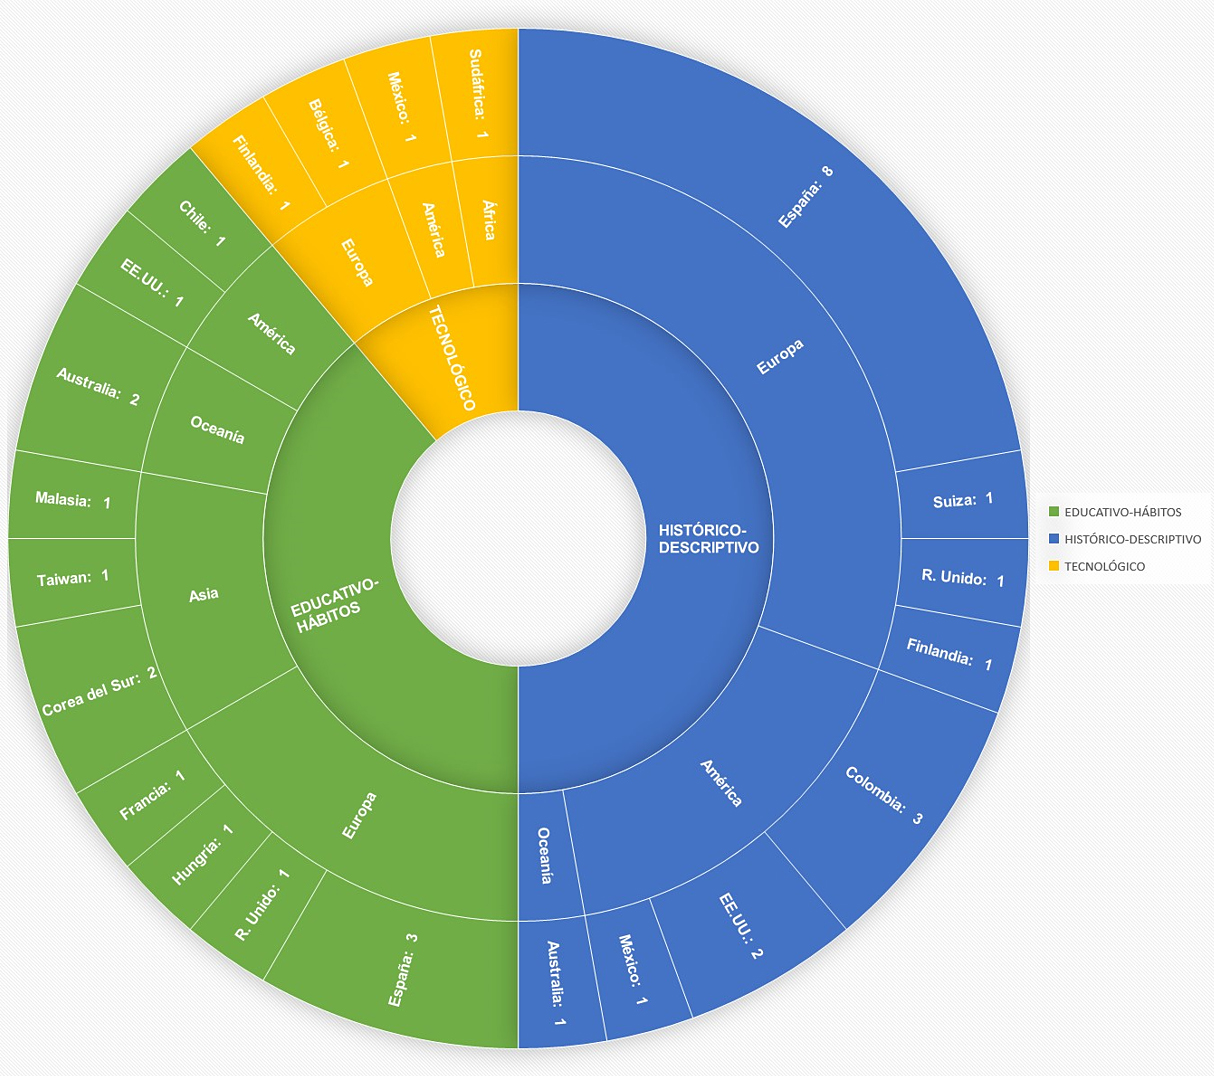
\includegraphics[width=\textwidth]{fig-003[1].jpg}
 \caption{Origen geográfico de las autorías según el ámbito de estudio.}
 \label{fig3}
 \source{elaboración propia.}
\end{figure}

Los datos recopilados ponen de relieve que son los países más desarrollados a nivel tecnológico o con un mayor índice de desarrollo los que encabezan los estudios. Por este motivo, Finlandia, Estados Unidos, Sudáfrica, Corea del Sur y Australia son los primeros del ranking. Esto revela que los países tecnológicamente más avanzados son además los que poseen una industria audiovisual más desarrollada, pues en el tema de las narrativas móviles ambas áreas se complementan. Asimismo, prevalecen aquellos estudios realizados en el ámbito anglosajón –incluidos Sudáfrica y Australia por la influencia que en ambos entornos tienen de Reino Unido-. La presencia es menor en Asia, lo que da a entender que el tema no tiene tanta visibilidad en los países enmarcados en otras culturas, aunque también aporten trabajos, sobre todo desde los enfoques histórico-descriptivo o educativo y relativo a los hábitos de consumo de los usuarios. 

\subsection{Colaboración entre universidades}
En cuanto a las instituciones donde se han gestado las investigaciones y las colaboraciones entre las universidades, los centros de investigación o las empresas (las grandes corporaciones de telefonía móvil), los artículos realizados por autores de universidades de un mismo país son más numerosos que los elaborados entre universidades de diferentes países. En Europa se da esta situación en España, con los trabajos de \textcite{adelantadomateu2011} –de la Universidad Politécnica de Valencia y de la Universidad de Valencia–, y de \textcite{feijoo2010} –de la Universidad Politécnica de Madrid y de la Universidad Nacional de Educación a Distancia (UNED)–, así como en Bélgica, con la investigación de \textcite{evens2011} –autores procedentes de la Ghent University y de la Katholieke Universiteit Leuven–, y Finlandia, país donde el trabajo de \textcite{jumiskopyykko2008} fue realizado entre la Tampere University of Technology y el Nokia Research Center, dando lugar a una de las aportaciones de carácter más técnico de la muestra. 

En el caso de América, estas colaboraciones se han producido en países como Colombia, con el artículo de \textcite{montoyabermudez2016} –realizado entre la Universidad Católica Popular de Risaralda, la Universidad de Antioquia y la Universidad Eafit–, y México, donde la investigación de \textcite{tamayofernandez2011} se acometió entre la Universidad Autónoma de Baja California y el Centro de Investigación Científica y de Educación Superior de Ensenada. Por su parte, en Asia existen tres casos. El primero de ellos es el de Corea del Sur, con el artículo de \textcite{shim2017}, acometido entre Korea Information Society Development Institute, Yonsei University y Ewha Womans University, y el de \textcite{do2009}, desarrollado entre cuatro instituciones de educación superior: Sookmyung Women’s University, Inha University, Kookmin University y Yonsei University. Asimismo, destacan Taiwan, donde la investigación de \textcite{su2015} fue realizada en Shu-Te University y National Yunlin University of Science and Technology, y Malasia, donde \textcite{wong2016} colaboraron desde Wawasan Open University, Universiti Tunku Abdul Rahman, University of Malaya y UCSI University. 

El único artículo del corpus realizado entre universidades de distintos países es el desarrollado por \textcite{varan2013} entre la Murdoch University, la Australian School of Management y la RMIT University –en Australia–, y la Florida State University y la Indiana University, en Estados Unidos. Aunque es el único caso, resulta significativo que incluya a seis universidades. 

Parece evidente que el objeto de estudio tiene interés dentro de cada país, pero no tanto de forma transversal entre países, de ahí que no existan muchos estudios longitudinales. Esto puede estar relacionado con que la mayoría de los trabajos son estudios de caso dentro de cada entorno, lo que hace difícil la comparación entre contextos.
Sin duda, los trabajos interfacultativos e internacionales son posibles y contribuirán al enriquecimiento de los resultados en el futuro.

\section{Discusión y conclusiones}
Las cuestiones planteadas en el análisis permiten conocer la dimensión investigadora del objeto de estudio a nivel global. Los artículos estudiados ofrecen información sobre las narrativas audiovisuales móviles, sus estructuras y su descripción, su origen y evolución, la percepción y los hábitos de consumo del usuario, la dimensión tecnológica de los dispositivos, las posibilidades del producto en el universo transmedia o el estado de la cuestión en distintos países, fundamentalmente durante la última década.  

\subsection{Ámbito temático y planteamiento metodológico}
La muestra analizada gira sobre varios ejes: el universo transmedia, su descripción y evolución histórica, la tecnología y la educación y hábitos de consumo, que a veces aparecen combinados. Todos estos ámbitos contribuyen a la configuración de los puntos clave de las narrativas audiovisuales móviles: en primer lugar, la descripción y contextualización de las moviseries vs. webseries como herederas directas de las series de televisión, a través de las cuales también han buscado su supervivencia \cite{adelantadomateu2011} tras una primera etapa de auge e independencia de las moviseries. En segundo lugar, el papel de las narrativas móviles como nuevas narrativas audiovisuales dentro del inabarcable universo transmedia. En tercer lugar, su aproximación al concepto de \emph{storytelling}, como forma narrativa a través de la cual pueden desarrollarse en el futuro si consiguen adaptar la tecnología a la forma de contar historias con un fin concreto más allá del entretenimiento, y que puede desarrollarse en ámbitos como la comunicación comercial, la salud o la educación \cite{lugmayr2017}. 

En cuanto al planteamiento metodológico de los artículos de la muestra predomina el carácter cualitativo frente al cuantitativo y, en concreto, los estudios de caso. Con esta metodología se han analizado series de ficción procedentes de moviseries, webseries o de la televisión, que han permitido conocer las estructuras narrativas y su lugar en el ámbito de los dispositivos móviles. El hecho de que algunas sean españolas y otras americanas o australianas ha evidenciado que la realidad española no es tan diferente de la de otros continentes. Estos estudios de caso han observado también el funcionamiento de los productos en distintos países, destacando Australia, Corea del Sur y México, con varias pesquisas, y Estados Unidos y Finlandia, pioneros en la materia, así como los hábitos de consumo de los usuarios. A este respecto, las experiencias desarrolladas en varios estados, especialmente de Asia, ofrecen datos valiosos sobre cómo los ciudadanos perciben los productos seriados de ficción en sus móviles y cómo actúan con estos dispositivos. Esta interacción es muy relevante, pues permite que los usuarios se familiaricen con el producto y que las corporaciones televisivas y móviles obtengan información para seguir con él o transformarlo. 

\subsection{Internacionalización}
En lo referente al origen y procedencia de la muestra analizada, destaca el nivel de internacionalización de la misma, procedente de un total de 16 países de todos los continentes. Además de Europa, con estudios de siete países, sobresalen América y Asia, con los trabajos realizados en cuatro y en tres países. Estos continentes constituyen los focos de interés más desarrollados a nivel mundial sobre el tema, respondiendo, además, a los principales centros de la industria audiovisual y de la telefonía móvil. Así, se constata que ambos universos empresariales están bastante vinculados y favorecen el desarrollo del objeto de estudio en sus respectivos continentes. En cada uno existe un país que lidera las investigaciones en este ámbito. En Europa, Finlandia se erige como el estado pionero en el origen y el desarrollo de los estudios, mientras que en América y en Asia son Estados Unidos y Corea del Sur, respectivamente, las naciones punteras. Por otra parte, África y Oceanía completan el marco investigador a nivel geográfico, con Sudáfrica y Australia. En este sentido, resulta bastante relevante el caso australiano, cuyas investigaciones sobre el tema se han centrado en el estudio de series \cite{monaghan2017} y en el lugar de la publicidad móvil en estos productos frente a soportes como la televisión \cite{varan2013}. 

En cuanto al idioma en el que se han publicado las investigaciones de la muestra, conviven dos tendencias, fruto también de haber realizado las búsquedas con palabras clave en español e inglés. Por una parte, existen numerosas publicaciones en español, donde, además de España, están las aportaciones originarias de México, Colombia y Chile, que contribuyen a favorecer la visibilidad de las mismas en todos los países hispanohablantes. Por otra parte, son cuantiosos los trabajos en inglés que están presentes tanto en Reino Unido, Estados Unidos, Sudáfrica o Australia, como en otros países que han optado por elegirlo ante su idioma propio. Así sucede con los artículos procedentes de Finlandia, Italia y Asia. 

\subsection{Perfil de las contribuciones}
En la mayoría de los casos, las investigaciones analizadas pertenecen al ámbito académico, pero también aparecen trabajos realizados de forma conjunta con institutos de investigación de alta especialización y con empresas de tecnología líderes en su sector. Este es el caso del Nokia Research Center, cuya colaboración en Finlandia con la Tampere University of Technology hizo posible el trabajo realizado por \textcite{jumiskopyykko2008}. De esta manera, destacan los trabajos colectivos realizados por autores que pueden no pertenecer a la misma Universidad y que incluso proceden de diferentes disciplinas. Esto confiere una dimensión más completa del objeto de estudio, al ofrecer diversos puntos de vista, y se advierte notablemente en los trabajos con enfoque tecnológico. Algunos artículos de Corea del Sur \cite{do2009} y de Malasia \cite{wong2016} se enmarcan en esta perspectiva al combinar el esfuerzo de más de dos universidades. No obstante, el perfil dominante corresponde a trabajos realizados por dos universidades de prestigio de un mismo país. 

Según el análisis realizado sobre las narrativas audiovisuales móviles orientadas a la creación de productos de ficción, resulta oportuno concluir que parece haber existido un vacío notable en los primeros años de este siglo, seguido del auge del tema entre 2007 y 2012, año en el que se produce un estancamiento. Hasta esta fecha, las investigaciones contribuyeron a la definición del fenómeno, explicando sus características específicas para los soportes móviles. Por otra parte, a partir de 2012, el concepto de moviseries se vio absorbido por el de webseries debido a los frenos tecnológicos existentes en todos los países. Así, las plataformas móviles se convirtieron en instrumentos para difundir contenidos ya existentes en la televisión, cuyo acceso se produjo a través de los soportes móviles. Aunque este hecho sucedió en todos los continentes, dada la globalización de los canales de comunicación, los diferentes estados han abordado el objeto de modo particular analizando sus propios casos.

La televisión en el móvil se empezó a truncar desde el principio, a nivel comercial, en la mayoría de los países europeos \cite{feijoo2010}, dado que su consumo dependía en buena medida de cuestiones culturales de cada país. Mientras en Finlandia o Corea del Sur tuvo bastante éxito, en otros países no terminó de calar, puesto que en los primeros años del lanzamiento de las moviseries existía de manera generalizada un rechazo por parte de los usuarios a pagar por los contenidos \cite{saez2010, urban2007}. Sin embargo, y a pesar del poco tiempo transcurrido, este panorama es muy diferente al actual, en el que impera el streaming y el video bajo demanda y en el que los usuarios pagan para disfrutar de series de ficción en plataformas como Netflix o HBO \cite{rayabravo2018}. Por ello, estos productos han ido apareciendo en otros formatos, como las webseries \cite{montoyabermudez2016}, sobre todo a raíz del desarrollo de la transmedialidad, presente en la retroalimentación mutua que existía ya desde el principio entre los contenidos de televisión, Internet y el teléfono móvil \cite{saez2010}. En este sentido, las moviseries como formato de ficción han experimentado un cierto retroceso. 

Se concluye que, aunque no se puede hablar actualmente de un escenario donde se puedan definir de modo particular las narrativas audiovisuales móviles, las investigaciones precedentes sientan las bases del objeto de estudio, pudiendo vislumbrar un futuro investigador que debe potenciar los siguientes aspectos: 
El desarrollo de investigaciones interuniversitarias que aporten comparativas en tiempo y forma entre países y que sienten las bases comunes de estas nuevas narrativas. 

La realización de investigaciones cuantitativas que permitan el análisis de un mayor número de variables a tener en cuenta en el desarrollo del objeto de estudio, teniendo en cuenta que la mayoría de los trabajos analizados se han elaborado a través de metodologías cualitativas y de estudios de caso.  

La profundización en el enfoque descriptivo e histórico que pareció dejarse relegado a un segundo plano tras los primeros años de estudio. La revitalización de este enfoque se puede justificar con el nacimiento de nuevos soportes móviles con características técnicas que permiten la instalación de aplicaciones específicas para el consumo de moviseries.

El desarrollo de las posibilidades que ofrecen las moviseries al mundo comercial, permitiendo su comercialización, por ejemplo, a través de bartering –o colaboración en la producción de un contenido de ficción de una marca comercial–, lo que podría desarrollarse a través de estrategias que utilicen \emph{storytelling}. Aquí se podrían enmarcar también los fashion films que crean las marcas de moda de lujo para transmitir el universo de cada marca, pues se trata de piezas audiovisuales de corta duración y estética muy cuidada, que recurren al \emph{storytelling}, y que podrían abordarse también de forma específica para móviles, enriqueciendo así su propio mapa transmedia. 

Proponer nuevas teorías que puedan ser debatidas desde la práctica conjunta y no relegar la investigación únicamente a los estudios de diferentes realidades o países. Así, investigar las narrativas audiovisuales móviles desde un enfoque multidisciplinar, más allá de las teorías de la Comunicación, o de la Educación, se hace necesario para  desarrollar nuevas investigaciones que las expliquen a nivel global. 

\section{Financiación}
Investigación financiada por la Junta de Extremadura (Consejería de Economía, Ciencia y Agenda Digital) y por la Unión Europea “Fondo Europeo de Desarrollo Regional. Una manera de hacer Europa”.


\printbibliography\label{sec-bib}
% if the text is not in Portuguese, it might be necessary to use the code below instead to print the correct ABNT abbreviations [s.n.], [s.l.] 
%\begin{portuguese}
%\printbibliography[title={Bibliography}]
%\end{portuguese}


%full list: conceptualization,datacuration,formalanalysis,funding,investigation,methodology,projadm,resources,software,supervision,validation,visualization,writing,review
\begin{contributors}[sec-contributors]
\authorcontribution{Valeriano Durán Manso}[conceptualization,datacuration,review,investigation,methodology]
\authorcontribution{María-Victoria Carrillo-Durán}[resources,conceptualization,review,methodology]
\authorcontribution{Javier Trabadela-Robles}[conceptualization,review,methodology,visualization]
\end{contributors}

\end{document}
